\chapter{Interazione Radiazione Materia}
Il tempo tipico di decadimento delle particelle dipende dal tipo di interazione:
\begin{itemize}
    \item Forte  < $10^{-22}s$
    \item Debole > $10^{-13}s$
    \item EM $10^{-20}-10^{-14}s$
\end{itemize}
La lunghezza percorsa da una particella prima di decadere è $l=\beta \gamma c \tau_0$ quindi possono essere misurate direttamente protoni, neutroni, elettroni,neutrini (elusivi) e muoni. I $\pi$ e i K possono essere rivelati direttamente ma anche decadere nel rivelatore.
\\
\\
\textbf{Proprietà misurabili} :
\begin{itemize}
    \item \textbf{Momento} : per particelle cariche misurabile tramite il raggio di curvatura in campo magnetico $$p=qRB$$ \begin{center}
        (R ha un segno per essere consistente con la direzione e con la carica)
    \end{center}
    \item \textbf{Carica} : Direzione della deflessione in campo magnetico
    \item \textbf{Energia}: Misurabile tramite la carica rilasciata o la luce prodotta in un calorimetro
    \item \textbf{Tempo di vita}: Ricostruendo il vertice del decadimento (geometricamente) si può ricavare il tempo in cui è decaduta
    \item \textbf{Velocità}: Tramite TOF, angolo Cherenkov o dal $\frac{dE}{dx}$
    \item \textbf{Massa}: Ottenibile da $m^2=E^2-p^2$ o da $p=m\beta/\sqrt{1-\beta^2} $
\end{itemize}

\section{Interazione di particelle cariche}
I meccanismi di interazione principali per le particelle cariche sono:
\begin{itemize}

    \item \textbf{Eccitazione/Ionizzazione}: Un atomo viene ionizzato rilasciando un $e^-$ poi collezionato per formare un segnale o viene prodotta luce tramite de eccitazione

    \item \textbf{Bremstrahlung}: Particella che viene deflessa dal campo EM nucleare e irraggia (*significativa solo per $e^+$ ed $e^{-}$: particelle leggere*)

    \item \textbf{Cherenkov}: Onda d'urto EM prodotta da particelle veloci

    \item \textbf{Radiazione di transizione}: Radiazione emessa quando una particella attraversa un mezzo con indice di rifrazione discontinuo (es. separazione tra vuoto e dielettrico). Questo accade perchè il campo elettrico longitudinale subisce un brusco riarrangiamento che ,in situazioni di energie molto alte, causa irraggiamento

    L'intensità della radiazione è $\propto \gamma$ quindi può essere usata per misurare velocità

\end{itemize}
\subsection*{Particelle massive}
\subsectionmark{Particelle massive}
\addcontentsline{toc}{subsection}{Particelle massive}
    \subsubsection*{Stopping power}
        Lo stopping power è definito come il $-dE/dx$ per unità di densità del materiale quindi è misurata in $MeV cm^2/g$  ed è espresso in funzione di $\beta \gamma=p/m$.
        \\
        Queste curve, se non normalizzate per la massa della particella, possono essere utili per fare particle identification poichè ogni particella segue una curva a se

        \begin{figure}[H]
            \centering
            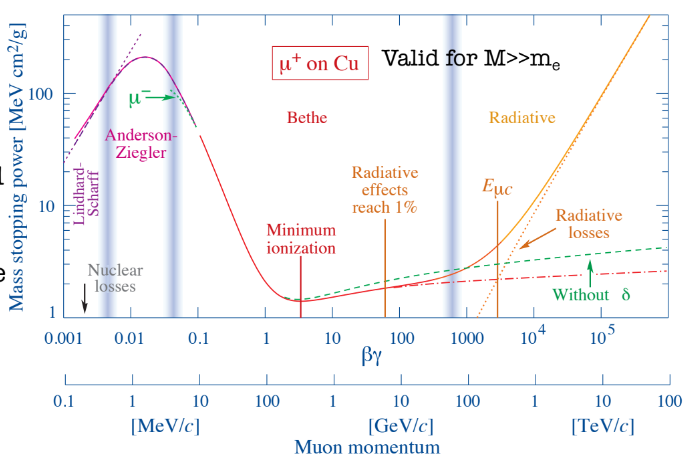
\includegraphics[width=0.8\textwidth,frame]{Chapters/images/Interazione_radiazione_materia/image-20220214171429817.png}
            \caption{Plot dello stopping power per particelle con $M>>m_e$ . Per elettroni e positroni domina Bremstrahlung.\\Possiamo distinguere 3 zone : zona di scattering elastico, di ionizzazione e di Bremstrahlung}
            \label{fig:betheblock}
        \end{figure}
    Analizziamo le diverse regioni della curva:
    \begin{itemize}
        \item Nella zona a più bassa energia (Lindhard-Scharff) si ha un andamento $\propto \beta$ dovuto a scattering elastico su nuclei

        \item La zona di Anderson-Ziegler è ottenuta empiricamente tramite fit su dati sperimentali per mettere un raccordo tra i modelli

        In questa zona si ha l' \textbf{effetto Barkas} che consiste in un minore stopping power per particelle negative (dovuto a fattori correttivi di ordine successivo)

        \item Nella zona di ionizzazione a basse energie si ha un andamento dominato da un fattore cinematico $\sim \beta^{-5/3} \sim \beta^{-2}$

        In questa zona la curva è molto sensibile a variazioni di $\beta$ quindi è possibile ricavare la velocità misurando il $dE/dx$

        \item A circa 3 - 4$\beta \gamma$ si ha il minimo di ionizzazione ed è $\sim 1-2 MeV cm^2/g$

        \item Dopo il minimo di ionizzazione si ha una risalita $\propto ln(\beta \gamma)^2$ dovuta all'estensione relativistica del campo elettrico trasversale ma per grandi $\beta \gamma$ il dielettrico viene polarizzato e si ha una saturazione (*effetto del $\delta$*)

        \item Al di sopra dell' \textbf{energia critica} dominano le perdite radiative ovvero la Bremstrahlung e altri processi minori
    \end{itemize}
Concentriamoci un attimo sulle perdite per \textbf{ionizzazione}

\begin{figure}[H]
    \centering
    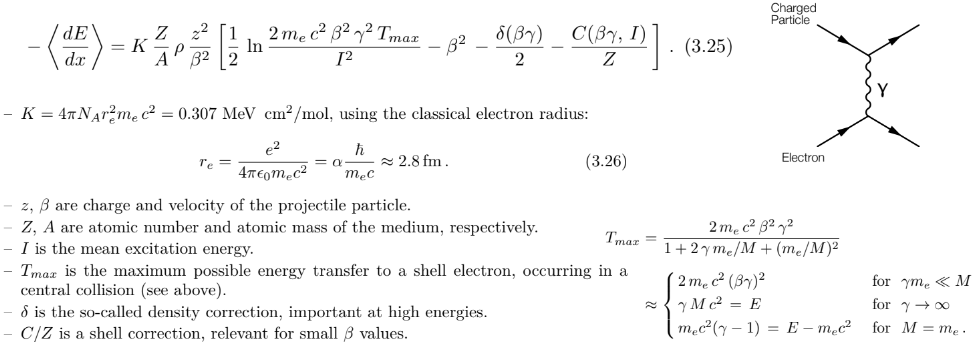
\includegraphics[width=0.95\textwidth,frame]{Chapters/images/Interazione_radiazione_materia/image-20220214173007634.png}
    \captionsetup{width=0.95\linewidth}
    \caption{Bethe-Block: dE/dx dovuta unicamente alla ionizzazione (zona centrale dello stopping power) (e alla radiazione Cherenkov). Non include nè le perdite per bremstrahlung (dominante ad alte energie) nè le perdite per radiazione di transizione}
    \label{fig:betheformula}
\end{figure}





\begin{minipage}{0.48\textwidth}
    \begin{figure}[H]
        \centering
        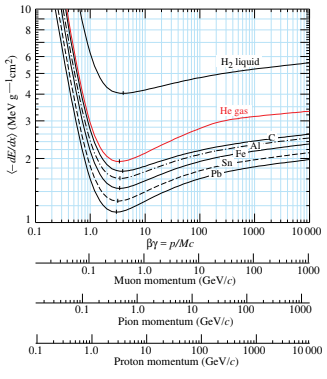
\includegraphics[width=\textwidth,frame]{Chapters/images/Interazione_radiazione_materia/image-20220214175355949.png}
        \captionsetup{width=\textwidth}
        \caption{A: Possiamo vedere come le curve sono essenzialmente indipendenti dal materiale salvo per l'idrogeno. Ricorda che sono normalizzate per la densità}
        \label{fig:}
    \end{figure}
\end{minipage} \hfill
\begin{minipage}{0.48\textwidth}

\begin{figure}[H]
    \centering
    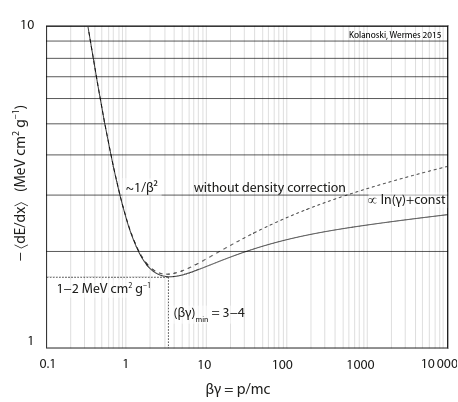
\includegraphics[width=\textwidth,frame]{Chapters/images/Interazione_radiazione_materia/image-20220214175429234.png}
    \captionsetup{width=\textwidth}
    \caption{B: Qui è possibile vedere meglio l'effetto del termine $\delta$ e della dipendenza logaritmica}
    \label{fig:}
\end{figure}

\end{minipage}
Alcune osservazioni sulla Bethe-Block (ionizzazione):
\begin{itemize}
    \item il fattore Z/A, per la formula semiempirica di massa, è più o meno sempre lo stesso $Z/A\sim 0.4$ tranne che per l'idrogeno $H_2$ dove è 1 (poichè non ha neutroni)
    \item A basse energie domina andamento $\sim \beta^{-2}$.
    \item La curva poi risale per 2 motivi:
    1. La massima energia trasferibile aumenta con $ \gamma$ (effetto cinematico)
    2. Il campo elettrico trasversale subisce un estensione per effetti relativistici anche se limitato dallo screening degli elettroni atomici che vengono polarizzati (termine $\delta$)
\end{itemize}

\subsubsection*{Picco di Bragg}

\begin{minipage}{0.55\textwidth}
    \begin{figure}[H]
        \centering
        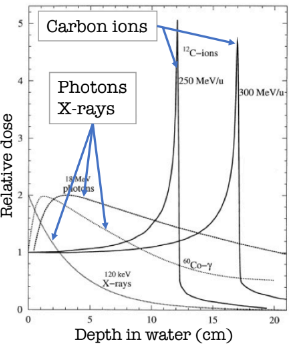
\includegraphics[width=0.75\textwidth,frame]{Chapters/images/Interazione_radiazione_materia/image-20220214183616196.png}
        \captionsetup{width=\textwidth}
        \caption{(La dose non è altro che E/M)}
        \label{fig:braggpeak}
    \end{figure}
\end{minipage} \hfill
\begin{minipage}{0.48\textwidth}
    Man mano che la particella perde energia lo stopping power aumenta. E' possibile ricostruire l'energia persa in funzione della penetrazione usando l'andamento $\beta^{-2}$ valido a basse energie

\end{minipage}

\subsubsection*{Elettroni delta}
Per trasferimenti di energia elevati possono essere strappati elettroni atomici che creano tracce secondarie (sufficientemente lunghe) nella stessa direzione della particella incidente (o comunque a piccoli angoli).
Se il detector non riesce a trattare adeguatamente questi elettroni si può avere un peggioramento della risoluzione spaziale (poichè la carica viene depositata più lontano dal punto di interazione) e fluttuazioni più grandi dello stopping power

\subsubsection*{Range}
Il range è la lunghezza percorsa dalla particella nel materiale $R=\int_{T_0}^0 (\frac{dE}{dx})^{-1} dT$ dove $T_0$ è l'energia cinetica iniziale della particella.

\begin{figure}[H]
    \centering
    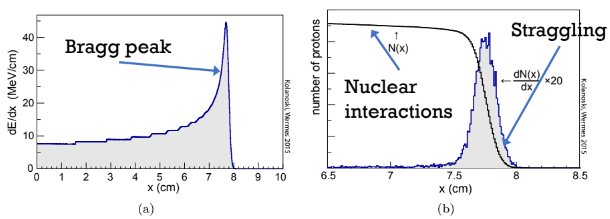
\includegraphics[width=0.8\textwidth,frame]{Chapters/images/Interazione_radiazione_materia/image-20220214185815482.png}
    \captionsetup{width=0.8\linewidth}
    \label{fig:straggling}
\end{figure}


\begin{minipage}{0.48\textwidth}
    \begin{figure}[H]
        \centering
        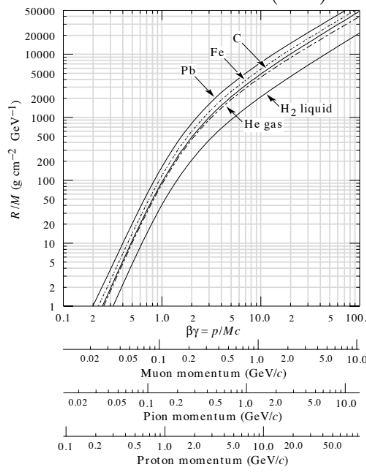
\includegraphics[width=\textwidth,frame]{Chapters/images/Interazione_radiazione_materia/image-20220216172742194.png}
        \captionsetup{width=\textwidth}
        \caption{Range normalizzato per la densità del materiale in funzione di $\beta \gamma$ . Plot utile per capire quanto materiale usare in un esperimento}
        \label{fig:}
    \end{figure}
\end{minipage} \hspace{1.cm}
\begin{minipage}{0.33\textwidth}
    Quando sono coinvolti fenomeni di assorbimento il numero di particelle decresce esponenzialmente (fotoni).
Quando sono coinvolte particelle cariche il numero di particelle rimane pressocchè costante. In figura si vede una lieve diminuzione dovuta a interazioni nucleari.
\\
\\
Si nota anche che il $dN/dx$ non è una delta ma ha una sua larghezza chiamata \textbf{straggling}: questo fenomeno è dovuto alle fluttuazioni statistiche dell'energia rilasciata nel materiale (vedi più avanti)
\\
\\
    Se si esprime l'integrale del range in funzione di $\gamma$ si ha $R=\frac{M}{z^2}f(\gamma_0)$ dove $\gamma_0$ è il $\gamma$ iniziale della particella e $f(\gamma_0)$ è una funzione indipendente dalle proprietà della particella (massa e carica) e dipende solo dal materiale. Quindi il range scala come $M/z^2$ (riferite alla particella)

\end{minipage}
\subsection*{Particelle poco massive ($e^{+} ; e^{-})$}
\subsectionmark{Particelle poco massive ($e^{+} ; e^{-})$}
\addcontentsline{toc}{subsection}{Particelle poco massive ($e^{+} ; e^{-})$}
Per le particelle cariche poco massive (elettroni e positroni) vale quanto detto sopra ma sono presenti dei fenomeni aggiuntivi:
\begin{itemize}


    \item La \textbf{bremstrahlug}
    \item Gli elettroni incidenti scatterano con elettroni atomici: Sono particelle identiche, interviene il principio di pauli
    \item Per positroni va considerata l'annichilazione con gli elettroni atomici

    Generalmente, oltre a prendere in considerazione la bremstrahlung, vanno considerati 2 regimi di energia:

    \item Quando i livelli energetici degli elettroni atomici NON possono essere trascurati si fa la media come nel caso di particelle massive
    \item Quando si hanno grandi trasferimenti di energia vengono considerati gli scattering Moller ($e^- e^- \to e^- e^-$) e Bhabha ($e^+ e^- \to e^+ e^-$)
\end{itemize}

\begin{figure}[H]
    \centering
    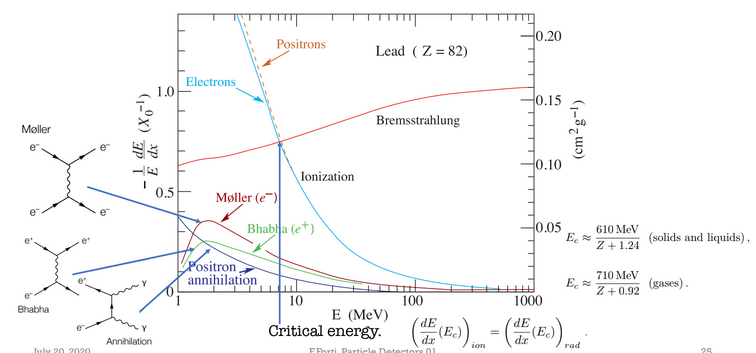
\includegraphics[width=0.8\textwidth,frame]{Chapters/images/Interazione_radiazione_materia/image-20220217021527324.png}
    \captionsetup{width=0.8\linewidth}
    \caption{Per particelle leggere il dE/dx è molto diverso in quanto la bremmstrahlung diventa dominante già sotto il GeV, nel piombo già a 7MeV \\ Anche qui si nota l'effetto per il quale la particella con carica negativa a basse energie perde un po' meno energia}
    \label{fig:electronloss}
\end{figure}
\subsubsection*{Bremstrahlung e lunghezza di radiazione}
Consiste nell'irragiamento dovuto alla deflessione dell'elettrone causata dal campo elettrico nucleare (scattering Rutherford con il nucleo)
\newline
L'energia emessa per una carica accelerata, sia nel limite classico che quantistico, è $dE/dt \propto \frac{1}{m^2}$

\begin{note}
    Ad altissime energie (es. LHC) la bremmstrahlung diventa rilevante anche per muoni e pioni
\end{note}

\[-\frac{dE}{dX} \Bigr|_\text{Brem} =\frac{E}{X_{0}} \quad \implies \quad  E(x) = E_{0} e^{\frac{-x}{X_{0} }} \]

\[\rho X_{0} =\frac{716.408 \: A \: \text{mol/g}}{Z(Z+1)\ln \frac{287}{\sqrt{Z} }} \frac{\text{g} }{\text{cm}^{2}  }
    \]
\(X_{0} \) $X_0$ è chiamata \textbf{lunghezza di radiazione} e corrispone alla lunghezza dopo il quale l'energia di un \textbf{elettrone} è ridotta di un frattore $1/e$ (per bremmstrahlung)

\begin{note}
    La lunghezza di radiazione è definita solo per elettroni in quanto per altre particelle molto energetiche come muoni le fluttuazioni di energia sono molto grandi e spesso sono associate a sciamature quindi parlare di perdita di energia come un processo uniforme e continuo è insensato
\end{note}
\begin{remark}

    Si noti la dipendenza (molto approssimativa a causa del log.) $-\frac{dE}{dx} \sim \propto E Z^2$

\end{remark}
Tipicamente la Bremmstrahlung viene emessa in avanti o comunque a piccoli angoli $\theta \sim1/\gamma=m/E$

\begin{figure}[H]
    \centering
    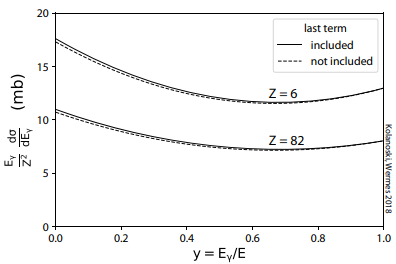
\includegraphics[height=3.2cm,frame]{Chapters/images/Interazione_radiazione_materia/image-20220220135143452.png}
    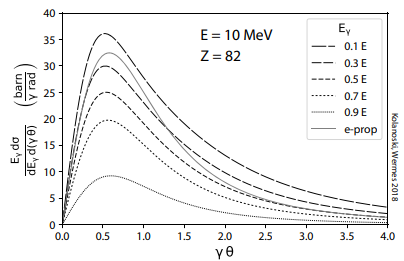
\includegraphics[height=3.2cm,frame]{Chapters/images/Interazione_radiazione_materia/image-20220220135223580.png}
    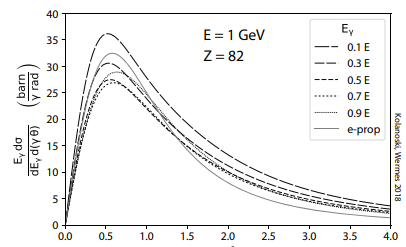
\includegraphics[height=3.2cm,frame]{Chapters/images/Interazione_radiazione_materia/image-20220220135322598.png}
    \captionsetup{width=0.9\linewidth}
    \caption{\textbf{A} : Spettro della Bremmstrahlung per C e Pb normalizzata per fattore $E_\gamma/Z^2$ \\ \textbf{B} ,\textbf{C} : distribuzione angolare della Bremmstrahlung a diverse energie}
    \label{fig:}
\end{figure}
Inoltre quando avviene Bremmstrahlung dobbiamo considerare vari possibili fenomeni:
\begin{itemize}
    \item Correzioni di Coulomb: Correzione dovuta all'interferenza della funzione d'onda della particella con il campo coulombiano

\item Suppressione dielettrica: Fotoni emessi a piccole energie vengono assorbiti nel materiali a causa della polarizzabilità del materiale causando una perdita di coerenza e un cutoff infrarosso nello spettro del fotone

\item La bremmstrahlung può avvenire anche con il campo elettrico degli elettroni atomici (basta sostituzione $Z^2 \to Z(Z+1)$)

\item Effetto LPM: Ad altissime energie (sopra il TeV) la Bremmstrahlung (e la produzione di coppie) è soppressa .
\end{itemize}
  Ad alte energie per energie perse piccole l'interazzione avviene su lunghe distanze. Se questa distanza è maggiore del cammino libero medio (distanza media tra 2 eventi successivi) la prima emissione interferisce con la seconda introducendo causando una soppressione nello spettro dei fotoni
\subsection*{Fluttuazioni statistiche}
\subsectionmark{Fluttuazioni statistiche}
\addcontentsline{toc}{subsection}{Fluttuazioni statistiche}
La Bethe block determina solo il $dE/dx$ medio ma in realtà l'energia rilasciata è soggetta a fluttuazioni.

L'energia persa $\Delta E$ in un tratto $\Delta x$ è la somma di tutti i processi di eccitazione/ionizzazione lungo il tratto percorso $\Delta E= \sum^N_{n=1} \delta E_n$.\\
Ci sono 2 contributi statistici:
\begin{itemize}
    \item Uno dovuto al numero di ionizzazioni/eccitazioni (conteggio)
    \item Uno dovuto all'energia emessa dal processo
    
    Queste fluttuazioni possono causare una serie di problemi
    
    \item \textbf{Incertezza sul momento}:Per ricostruire il momento di una particella solitamente si usa la Bethe Block per capire quanta energia ha perso nel detector ma le fluttuazioni statistiche introducono un'incertezza sull'energia persa e quindi anche sul momento
    \item \textbf{Incertezze nel PID} poichè la particle identification si fa soprattutto tramite le misure del $dE/dx$ è introdotta un incertezza anche su questo
    \item \textbf{Incertezze nel tracking}: I tracker sono solitamente sottili quindi soffrono delle fluttuazioni poissoniane. Inoltre la risoluzione spaziale è ulteriormente ridotta dagli elettroni delta che possono anche causare ionizzazioni secontarie
    
\end{itemize}

\subsubsection*{Fluttuazioni del numero di processi}
E' una fluttuazione di tipo \textbf{Poissoniano}, rilevante soprattutto in detector sottili (molto usati nel tracking) e l'incertezza relativa è
\[\frac{\sigma(\Delta E)}{\Delta E}\sim\frac{1}{\sqrt{N}}\]

\begin{remark}

    In caso di rivelatore spesso 1cm di Argon questa incertezza è del 10%
\\
    I rivelatori a semiconduttore invece necessitano energie molto più basse per produrre una coppia elettrone lacuna quindi vengono creati molti più elettroni e l'incertezza è molto ridotta rispetto i rilevatori a gas

\end{remark}

\subsubsection*{Fluttuazioni dell'energia rilasciata}
Dalla distribuzione angolare degli elettroni emessi nel processo di ionizzazione si trova che tra un valore $\delta E_{min}$ (dato dall'energia di ionizzazione dell'atome) e un valore $\delta E_{max}$ (dato da constraint cinematici) la distribuzione di $\delta E$ ha un andamento $\sim 1/(\delta E)^2$ .
\\
Il massimo della distribuzione si ha intorno a $\delta E_{min}$ ma ricordiamo che per energie più alte si presenta il problema degli elettroni delta

\subsubsection*{Distribuzione di Landau-Vavilov}

Generalmente le fluttuazioni nell'energia rilasciata portano a una distibuzione asimmetrica composta da una parte gaussiana (dovuta a piccole perdite di energia) e una lunga coda (per grandi perdite di energia)

\begin{note}
    A causa dell'asimmetria della distribuzione il valore più probabile di energia rilasciata NON è quello che vediamo nella Bethe Block (che è la media) che è un po' più alto della moda della distribuzione
\end{note}
Il primo a trovare una distribuzione fu \textbf{Landau} sotto le seguenti ipotesi:
\begin{itemize}
    \item $lim_{k \to0} T_{max}= +\infty$
    \item Gli elettroni sono trattati come quasi liberi, sono trascurati gli effetti di legame per bassi valori dell'energia trasferita
    \item La perdita di energia della particella nel mezzo può essere trascurata
\end{itemize}

\[
\begin{aligned}
    f_L(\lambda)=\frac{1}{\pi}\int_0^\infty e^{-t ln (t)-\lambda t }\sin (\pi t) dt
\\
\;\;\lambda=\frac{\Delta E -\Delta E_w}{\xi} \;\;
\\
\;\;\Delta E_w=\text{Massimo della distr.}
\end{aligned}\]
La forma della distribuzione dipende dal parametro $k=\xi/T_{max}$ dove $T_{max}$ è l'energia cinetica massima cedibile a un elettrone e $\xi \propto \rho\frac{Z}{A}\frac{z^2}{\beta^2} \Delta x$  è il fattore moltiplicativo presente nella bethe block quindi essezialmente $\xi \simeq dE/dx$ (almeno concettualmente, nell'andamento)
\begin{itemize}
    \item \textbf{k grande implica distribuzione simmetrica (Gaussiana)}
\item \textbf{k piccolo implica distribuzione asimmetrica}

\end{itemize}
La distribuzione di landau è un'ottima \textbf{approssimazione per piccoli valori di k}

\begin{minipage}{0.48\textwidth}
    \begin{figure}[H]
        \centering
        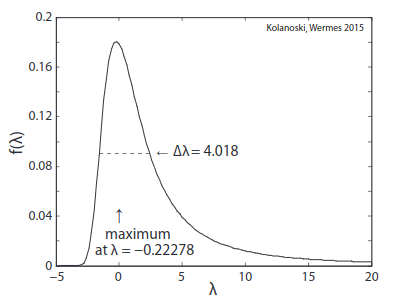
\includegraphics[width=\textwidth,frame]{Chapters/images/Interazione_radiazione_materia/image-20220216191943021.png}
        \captionsetup{width=\textwidth}
        \caption{Distribuzione di Landau. Il $\Delta \lambda$ è la larghezza a metà altezza}
        \label{fig:landau}
    \end{figure}
\end{minipage} \hspace{0.4cm}
\begin{minipage}{0.4\textwidth}
\begin{remark}
    La landau può essere approssiamata dalla distribuzione di Moyal $f(\lambda)=\frac{1}{\sqrt{2\pi}}e^{-0.5(\lambda+e^{-\lambda})}$ 
In questo caso però $\lambda$ perde il senso fisico che ha nella landau per questo è preferibile usare la Landau
\end{remark}
\textbf{Vavilov}  generalizzò la distribuzione anche per grandi valori di k ma comunque mantenendo l'assunzione che gli effetti di legame siano trascurabili per piccoli davoli di energia trasferita.
Questa distribuzione ha 2 parametri aggiuntivi rispetto alla distribuzione di Landau
\end{minipage}
\begin{details}
    Senza entrare nel dettaglio la Vavilov è definita tramite una trasformata di Laplace
\end{details}
\subsubsection*{Soppressione delle fluttuazioni}

La fluttuazioni possono essere ridotte se la moda della distribuzione può essere usata come uno stimatore dell'energia persa al posto della media poichè la moda gode di uno stimatore migliore (La distribuzione ha una coda molto lunga quindi la media aritmetica potrebbe avere una varianza molto grande rispetto alla moda soprattutto ad alte energie)

\hspace{-30pt}
\begin{minipage}{0.52\textwidth}
    \begin{figure}[H]
        \centering
        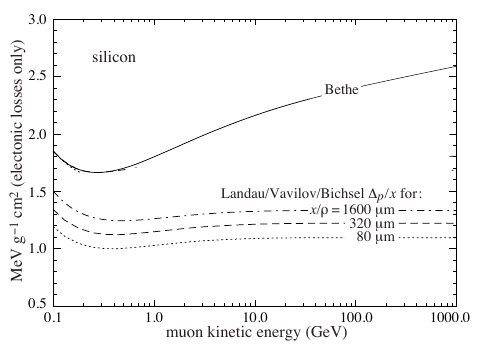
\includegraphics[width=\textwidth,frame]{Chapters/images/Interazione_radiazione_materia/image-20220217014236788.png}
        \captionsetup{width=\textwidth}
        \caption{Le curve tratteggiate sono relative alla moda invece che alla media. Si nota che ad alte energie la media sale molto di più rispetto alla moda}
        \label{fig:landaumode}
    \end{figure}
\end{minipage} \hfill
\begin{minipage}{0.48\textwidth}
    Altri metrodi per eliminare incertezze sono:
\begin{itemize}
    \item Escludere gli elettroni deltra dalle misurse (Possibile in cloud/bubble chamber e in layer indipendenti molto sottili di un detector)
    \item Usare una media troncata scartando i valori più alti e più bassi (Stima più robusta)
    \item Ricostruire l'energia persa dalla particella durante il suo percorso e non solo alla fine (Utile nella misura del momento.)
\end{itemize}


\end{minipage}
\subsection*{Multiplo Scattering}
\subsectionmark{Multiplo Scattering}
\addcontentsline{toc}{subsection}{Multiplo Scattering}
In un materiale possono avvenire scattering multipli. Questi causano un'incertezza nella direzione della particella.
La distribuzione angolare dell'angolo di scattering medio può essere ben approssimata  con una gaussiana (per limite centrale)
\begin{remark}
    per un numero finito e fissato di scattering c'è distribuzione di Moliere che però predice probabilità più alte per grandi angoli come Rutherford
\end{remark}
\begin{figure}[H]
    \centering
    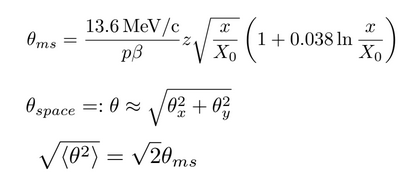
\includegraphics[width=0.8\textwidth,frame]{Chapters/images/Interazione_radiazione_materia/image-20220217025524958.png}
    \captionsetup{width=0.8\linewidth}
    \caption{Deviazione standard dell'angolo di scattering nell'approssimazione gaussiana a piccoli angoli (valida al di sopra dei 20MeV)}
    \label{multiplescattering}
\end{figure}
\begin{figure}[H]
    \centering
    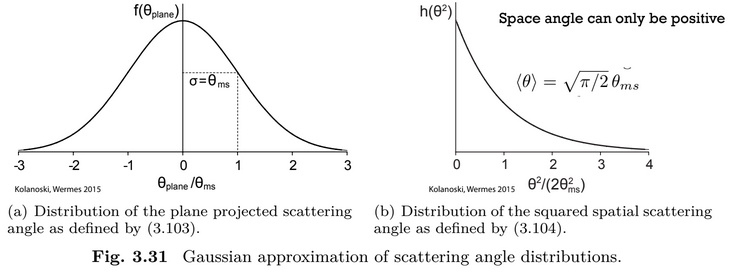
\includegraphics[width=0.8\textwidth,frame]{Chapters/images/Interazione_radiazione_materia/image-20220217030024845.png}
    \captionsetup{width=0.8\linewidth}
    \caption{NB: l'angolo ha un segno.\\Se si considera il valore assoluto dell'angolo la distribuzione cambia}
    \label{fig:mmscatteringradius}
\end{figure}
\subsection*{Radiazione Cherenkov}
\subsectionmark{Radiazione Cherenkov}
\addcontentsline{toc}{subsection}{Radiazione Cherenkov}
La radiazione Cherenkov avviene quando una particella carica attraversa un mezzo a una velocità maggiore della velocità della luce nello stesso mezzo causando un'onda d'urto luminosa.
\\
Quello che viene prodotto è un cono luminoso con una apertura angolare di $\cos(\theta_c)=\frac{1}{n\beta}$ , questo significa che la luce cherenkov può essere usata per trovare $\beta$ (e se si è misurato in qualche altro modo il momento anche la massa) o come threshold in quanto viene emessa solo per $\beta>1/n$
\\
L'energia persa per radiazione cherenkov è solitamente molto bassa e trascurabile (Comunque inclusa nella bethe bloch nelle perdite radiative)
\subsection*{Misture}
\subsubsectionmark{Misture}
\addcontentsline{toc}{subsection}{Misture}
Soprattutto nei detector gassosi possono essere presenti più materiali insieme
\begin{figure}[H]
    \centering
    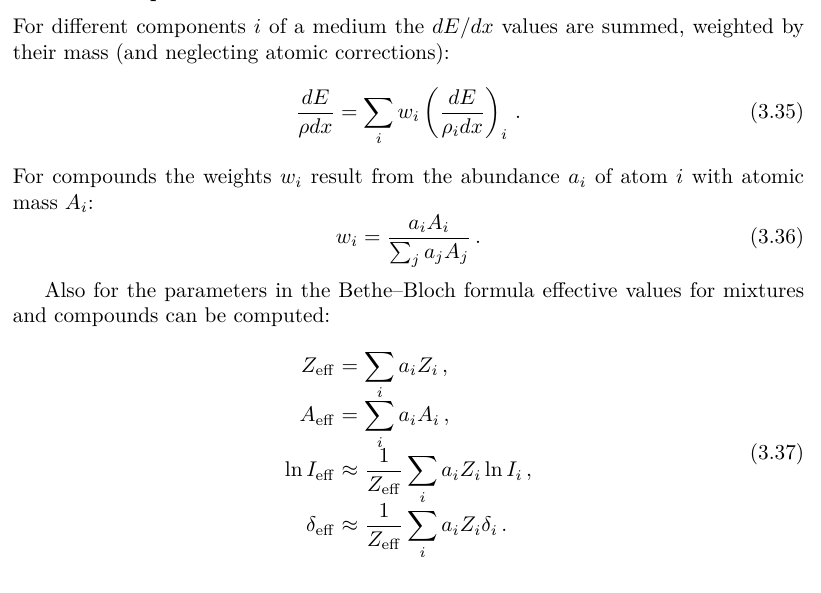
\includegraphics[width=0.8\textwidth,frame]{Chapters/images/Interazione_radiazione_materia/image-20220217042603821.png}
    \captionsetup{width=0.8\linewidth}
    \label{fig:misture}
\end{figure}
Per la lunghezza di radiazione invece $\frac{1}{\rho X_0}|_{\text{eff.}}=\sum_i \frac{1}{\rho_i X_{0_i}}$
